\documentclass{article}
\usepackage{tikz}
\usetikzlibrary{positioning}

\begin{document}

\begin{figure}[h]
    \centering
    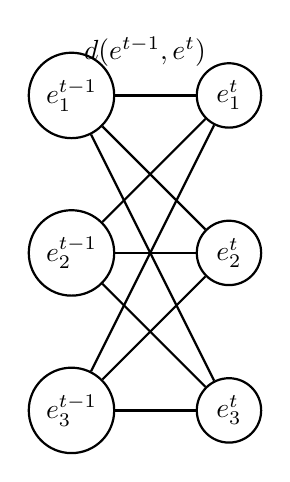
\begin{tikzpicture}[node distance={20mm}, thick, main/.style = {draw, circle}]
        \node[main] (1) {$e_1^{t-1}$};
        \node[main] (2) [below of=1] {$e_2^{t-1}$};
        \node[main] (3) [below of=2] {$e_3^{t-1}$};
        \node[main] (4) [right of=1] {$e_1^{t}$};
        \node[main] (5) [right of=2] {$e_2^{t}$};
        \node[main] (6) [right of=3] {$e_3^{t}$};

        \draw (1) -- (4);
        \draw (1) -- (5);
        \draw (1) -- (6);
        \draw (2) -- (4);
        \draw (2) -- (5);
        \draw (2) -- (6);
        \draw (3) -- (4);
        \draw (3) -- (5);
        \draw (3) -- (6);

        \node at (current bounding box.north) {$d(e^{t-1}, e^{t})$};
    \end{tikzpicture}
    \caption{Illustration of bipartite matching for computing the similarity between sense clusters' centroids $p_1^t$ and $p_1^{t-1}$. Here, $\{e_i^{t}\}_{i=1}^3$ indicates the representative embeddings of three semantically nearest neighboring words to $p_1^t$. The same applies to $\{e_i^{t-1}\}_{i=1}^3$ and $p_1^{t-1}$.}
    \label{fig:bipartite_matching}
\end{figure}

\end{document}